%
% $XORP: xorp/docs/snmp/snmp_overview.tex,v 1.33 2008/12/30 00:36:12 jtc Exp $
%

\documentclass[11pt]{article}

%\usepackage[dvips]{changebar}

\usepackage{subfigure}
\usepackage{fullpage}
\usepackage{setspace}
\usepackage{times}
\usepackage{latexsym}
\usepackage{epsfig}
\usepackage{graphicx}
\usepackage{xspace}
\usepackage{color}
\usepackage{amsmath}
\usepackage{rotating}
\usepackage{moreverb}
\usepackage{listings}
\usepackage{alltt}
\usepackage{stmaryrd}
%\usepackage[dvipdf]{graphics}
%\usepackage[dvips]{graphicx}
%\usepackage{xorp}

\definecolor{gray}{rgb}{0.5,0.5,0.5}
\newcommand{\etc}{\emph{etc.}\xspace}
\newcommand{\ie}{\emph{i.e.,}\xspace}
\newcommand{\eg}{\emph{e.g.,}\xspace}
%\newcommand{\comment}[1]{{\color{gray}[\textsf{#1}]}}
%\newcommand{\comment}[1]{}

% Changebar stuff
% \newenvironment{colorcode}{\color{blue}}{}
% \renewcommand{\cbstart}{\begin{colorcode}}
% \renewcommand{\cbend}{\end{colorcode}}

% \pagestyle{empty}

\begin{document}

\title{XORP SNMP Agent \\
\vspace{1ex}
Version 1.6}
\author{ XORP, Inc.					\\
         {\it http://www.xorp.org/}			\\
	 {\it feedback@xorp.org}
}
\date{January 7, 2009}

\maketitle


%%%%%%%%%%%%%%%%%%%%%%%%%%%%%%%%%%%%%%%%%%%%%%%%%%%%%%%%%%%%%%%%%%%%%%%
\section{Introduction}

The SNMP standards \cite{STD0062} define the protocol used to communicate
between SNMP managers and agents, as well as the structure of the management
information being accessed (MIB).  This document describes how XORP runtime data
is made accessible to the SNMP agent, how it is decomposed in separate MIB
modules, and how those modules are loaded/unloaded at runtime.  Also, a MIB
development framework is presented, which provides unified process to those
writing new MIB modules for XORP.

%%%%%%%%%%%%%%%%%%%%%%%%%%%%%%%%%%%%%%%%%%%%%%%%%%%%%%%%%%%%%%%%%%%%%%%
\section{The SNMP agent}

XORP uses the extensible SNMP agent included in the Net-SNMP package
\cite{net-snmp}.  Net-SNMP provides tools and libraries supporting the Simple
Network Management Protocol.  The package is comprised of an extensible agent
(\texttt{snmpd}), an SNMP library and a set of command line tools to
communicate with SNMP agents and managers. 

Management information is viewed as a collection of managed objects, residing
in a virtual information store, termed the Management Information Base (MIB).
All managed objects in the MIB are arranged in a hierarchical or tree
structure.  Collections of related objects are defined in MIB modules.  These
modules are written in the SNMP data definition language, a subset of Abstract
Syntax Notation One (ASN.1).  New MIB modules that extend the Internet-standard
MIB are continuously being defined by various IETF working groups.  

In the context of this document, we'll extend the term MIB module to include
the part of the code that instantiates the objects declared in the MIB
definition file.  Thus a MIB module consists of:

\begin{description}

  \item[MIB module definition file] This file is written in ASN.1 language,
  and is typically published as an RFC.

  \item[MIB module source code] One or more source files that implement the
  data access routines that allow the SNMP agent to read or modify XORP's
  configuration settings. 

\end{description} 

The oldest version of Net-SNMP that was tested with XORP is 5.0.6.  If an
older version is detected by our \texttt{configure} script, XORP MIB modules
will not be built.

%%%%%%%%%%%%%%%%%%%%%%%%%%%%%%%%%%%%%%%%%%%
\subsection{Dynamically loadable MIB modules}
\label{sec:MIB_module_format}

One of the guiding principles in XORP design is extensibility.  Protocols are
implemented as independent Unix processes that may come and go.  Each protocol
will have one or more associated MIB modules, so those modules should be made
available to the SNMP agent without requiring recompilation.  Net-SNMP supports
this strategy by allowing MIBs to be implemented as shared objects.  If your
system supports shared libraries, Net-SNMP will be compiled with support for
dynamically loadable MIB modules by default.  You can test if your Net-SNMP
installation supports that option by looking for \texttt{dlmod} in the list
printed by the command:

\begin{verbatim}
$ net-snmp-config --snmpd-module-list
\end{verbatim}


There are three methods for loading/unloading MIB modules:  

\begin{enumerate}
  \item Using the dlmod directive in snmpd.conf 
  \item Sending SNMP set requests to the agent
  \item Using XORP's IPC methods (XRLs)
\end{enumerate}

The first option can only be used to load modules at startup.  This is what the
man page for snmpd.conf tells you...

\begin{verbatim}
DYNAMICALLY LOADABLE MODULES
	If the agent is built with support for the UCD-DLMOD-MIB it is  capable
	of  loading  agent MIB modules dynamically at startup through the dlmod
	directive and during runtime through use  of  the  UCD-DLMOD-MIB.   The
	following directive loads the shared object module file PATH which uses
	the module name prefix NAME.

	dlmod NAME PATH
\end{verbatim}


To load MIBs using SNMP requests, a new row must be added to
UCD-DLMOD-MIB::dlmodTable.  This involves finding an unused index to the table,
setting the values of dlmodName and dlmodPath for that row, and finally setting
the column dlmodStatus to 'load'.  These steps are captured in the following
lines:

\begin{verbatim}
$ snmpwalk localhost UCD-DLMOD-MIB::dlmodTable
UCD-DLMOD-MIB::dlmodName.1 = STRING: xorp_if_mib_module
UCD-DLMOD-MIB::dlmodPath.1 = STRING: /scratch/xorp/mibs/xorp_if_mib_module.so
UCD-DLMOD-MIB::dlmodError.1 = STRING:
UCD-DLMOD-MIB::dlmodStatus.1 = INTEGER: loaded(1)

$ snmpset localhost UCD-DLMOD-MIB::dlmodStatus.2 i create
UCD-DLMOD-MIB::dlmodStatus.2 = INTEGER: create(6)

$ snmpset localhost UCD-DLMOD-MIB::dlmodName.2 s "bgp4_mib_1657"  \ 
>    UCD-DLMOD-MIB::dlmodPath.2 s "/scratch/xorp/mibs/bgp4_mib_1657.so"
UCD-DLMOD-MIB::dlmodName.2 = STRING: bgp4_mib_1657
UCD-DLMOD-MIB::dlmodPath.2 = STRING: /scratch/xorp/mibs/bgp4_mib_1657.so

$ snmpset localhost UCD-DLMOD-MIB::dlmodStatus.2 i load
UCD-DLMOD-MIB::dlmodStatus.2 = INTEGER: load(4)

$ snmpwalk localhost UCD-DLMOD-MIB::dlmodTable
UCD-DLMOD-MIB::dlmodName.1 = STRING: xorp_if_mib_module
UCD-DLMOD-MIB::dlmodName.2 = STRING: bgp4_mib_1657
UCD-DLMOD-MIB::dlmodPath.1 = STRING: /scratch/xorp/mibs/xorp_if_mib_module.so
UCD-DLMOD-MIB::dlmodPath.2 = STRING: /scratch/xorp/mibs/bgp4_mib_1657.so
UCD-DLMOD-MIB::dlmodError.1 = STRING:
UCD-DLMOD-MIB::dlmodError.2 = STRING:
UCD-DLMOD-MIB::dlmodStatus.1 = INTEGER: loaded(1)
UCD-DLMOD-MIB::dlmodStatus.2 = INTEGER: loaded(1)
\end{verbatim}

So far we've seen how to load MIBs when the agent is started, and at runtime
using SNMP requests.  But XORP processes communicate to each other via XRLs,
and it would be much more convenient for a process to be able to use the same
mechanism to communicate with the SNMP agent.  For this reason each MIB module
should implement an Xrl target.  The module \texttt{xorp\_if\_mib\_module}
implements an XRL interface that allows loading and unloading MIBs.  These are
the XRLs to use for that: 

\begin{ttfamily}
\begin{verbatim}
finder://xorp_if_mib/xorp_if_mib/0.1/load_mib?mod_name:txt&abs_path:txt
finder://xorp_if_mib/xorp_if_mib/0.1/unload_mib?mib_index:u32
\end{verbatim}
\end{ttfamily}

Dynamically loadable MIB modules written for the main SNMP agent can also be
loaded by an SNMP sub-agent that communicates with the master agent via the
AgentX protocol (\cite{AgentX}).  This should be useful in the event that you
configure XORP to run distributed across multiple hosts but with one 
master SNMP agent.  


%%%%%%%%%%%%%%%%%%%%%%%%%%%%%%%%%%%%%%%%%%%%%%%%%%%%%%%%%%%%%%%%%%%%%%%
\section{Connecting Net-SNMP with XORP}

We have written a special MIB module (\texttt{xorp\_if\_mib\_module}) that
coordinates the communication between \texttt{snmpd} and XORP processes.  This
module provides several classes that allow XORP MIB modules to be architected
as if they were each executed as independent processes (although they all run
in \texttt{snmpd}'s process space).  This should make MIB module design much
easier to someone already familiar with the architecture of XORP processes.
 
The class that does all the synchronization between XORP and Net-SNMP 
is SnmpEventLoop, a subclass of EventLoop.  This singleton class is
responsible for registering XORP event's with \texttt{snmpd}, so that the agent
can respond to XORP activity.  Once this class is instantiated by
\texttt{xorp\_if\_mib\_module}, it can be used by all the other MIB modules as
if it was their own EventLoop.  Without it, MIB modules could not respond to
XORP events, this is why this module must be loaded before any other, and
should be the last XORP MIB module to be unloaded \footnote{There is a second
reason for this requirement.  Some runtime loaders will unload a dynamically
linked library when the module that first loaded it disappears.  In that case,
unloading \texttt{xorp\_if\_mib\_module} will also unload
\texttt{libnetsnmpxorp.so} which is needed by \emph{all} XORP modules.  As you
can imagine, that causes problems...}.  Typically you would use the
\texttt{snmpd.conf} file to load it at start up time.  

The XORP interface MIB module also implements the XRL target (\cite{xorp:xrl})
that allows the loading and unloading of other MIB modules.  


Figure \ref{fig:xorp-if-diag} illustrates the functionality implemented by 
\texttt{xorp\_if\_mib\_module}.

\begin{figure}
  \begin{center}
    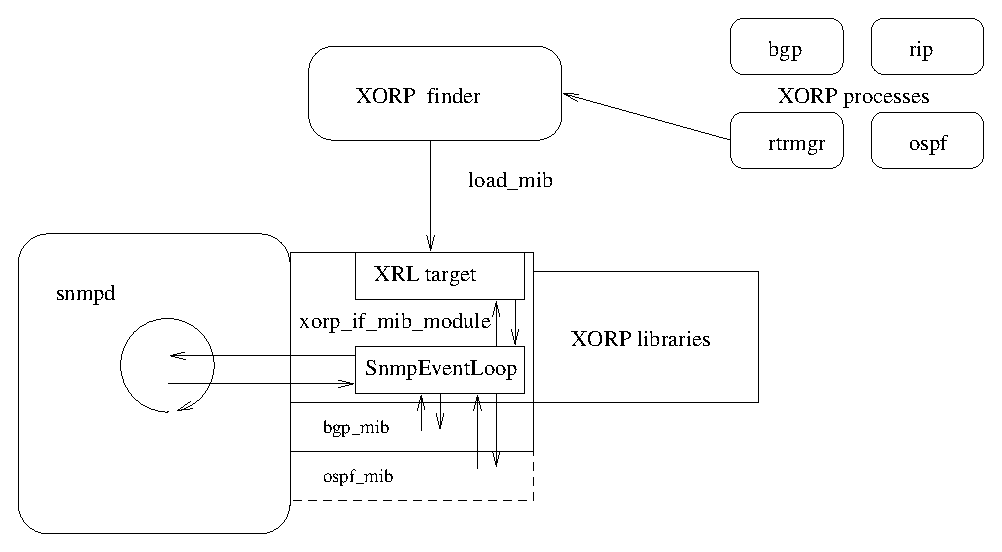
\includegraphics[width=1\textwidth]{figs/snmp_fig2}
  \end{center}
  \caption{Functionality of xorp\_if\_mib\_module}
  \label{fig:xorp-if-diag}
\end{figure}

%%%%%%%%%%%%%%%%%%%%%%%%%%%%%%%%%%%%%%%%%%%
\subsection{Modifying XORP's configuration from within a MIB module}

MIB modules use XORP's IPC library \cite{xorp:xrl} to communicate to XORP
processes.  Each MIB module has the responsibility to pull the relevant
management information from the appropriate process (\eg BGP MIB data from BGP
process).  For that effect, the MIB module must use the XRL Interface
supported by the XRL targets it needs to communicate to (see
\cite{xorp:xrl_interfaces} for details on how to subclass XRL Interface Client
classes).  MIB modules, though, MUST not modify any configuration settings by
accessing the process directly.  The current state of configuration is
maintained by the router manager process, so bypassing it would cause the real
and the recorded configurations to be out of sync.  Instead, configuration
changes should be requested to the router manager via configuration commands,
that is, XRLs such as the ones appearing in the template files (see
xorp/etc/templates/*.tp).

Figure \ref{fig:mib-class-diag} illustrates how the MIB modules should read and
change XORP configuration.

\begin{figure}
  \begin{center}
    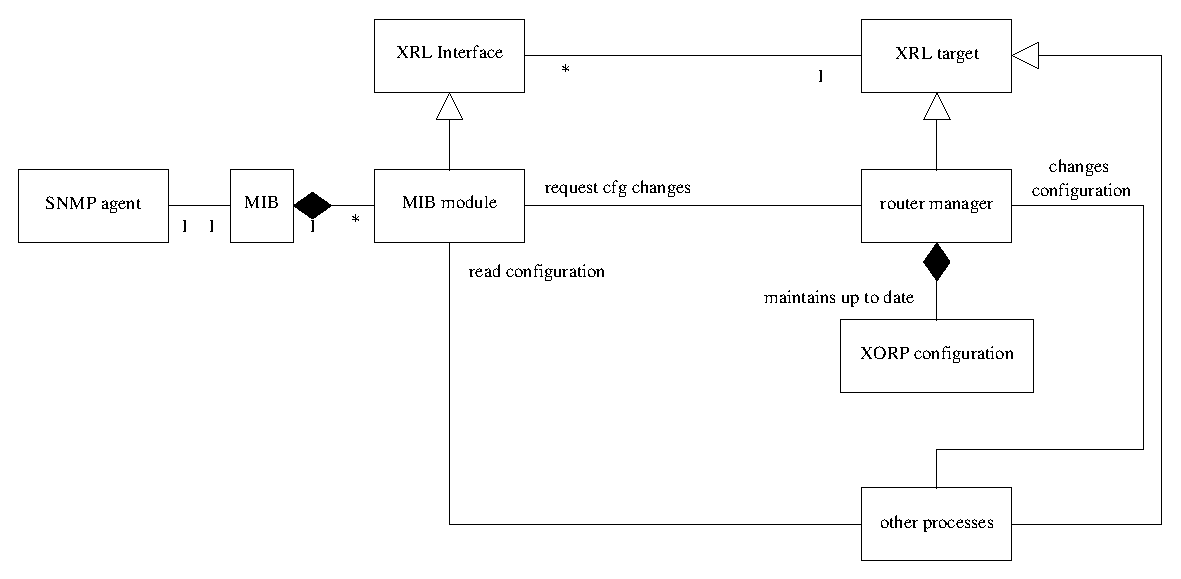
\includegraphics[width=1\textwidth]{figs/snmp_fig1}
  \end{center}
  \caption{MIB module interactions with the router manager}
  \label{fig:mib-class-diag}
\end{figure}

%%%%%%%%%%%%%%%%%%%%%%%%%%%%%%%%%%%%%%%%%%%%%%%%%%%%%%%%%%%%%%%%%%%%%%%
\section{A reference implementation of a MIB module}

So far we've talked Net-SNMP configuration.  In this section we'll cover
how to write a MIB module.  Currently (July 2008) we provide a full
implementation of RFC 1657, the MIB for BGP4.  You will find the MIB module
files in xorp/mibs/bgp4\_mib\_1657*.  What follows is a description the tools
and process followed to implement this module.  You should refer to the
kdoc documentation as well as the source itself for more details.   

%%%%%%%%%%%%%%%%%%%%%%%%%%%%%%%%%%%%%%%%%%%
\subsection{The textual MIB definition file}

The first step to write a MIB module should be writing or getting the ASN.1 MIB
definition file.  If you are implementing an existing protocol, chances are
that there is already a published RFC with the MIB definition for it.  In this
section we'll use BGP4-MIB to illustrate the process of writing a MIB module,
which is published in RFC 1657 and you will find in
xorp/mibs/textual/BGP4-MIB.txt.

You will also have to  make your textual MIB file accessible to the Net-SNMP
tools.  See the \texttt{mibs} and \texttt{mibdirs} directives in the man page
snmp.conf(5).  One way to do this is to copy our MIB onto the default
directory, and then set the MIBS environment variable:

\begin{verbatim}
$ cp BGP4-MIB.txt /usr/local/share/snmp/mibs
$ export MIBS=+BGP4-MIB
\end{verbatim}

%%%%%%%%%%%%%%%%%%%%%%%%%%%%%%%%%%%%%%%%%%%
\subsection{Net-SNMP handlers}

Net-SNMP 5.x.x uses handlers to process SNMP requests.  When a MIB module is
loaded, it registers one or more handlers (callbacks) on a given OID in the OID
tree.  When a request arrives for that OID subtree, the registered handlers
are called in sequence until the request is fully processed.  There are
multiple pre-written handlers (helpers, in Net-SNMP nomenclature) that deal
with certain parts of the processing.

%%%%%%%%%%%%%%%%%%%%%%%%%%%%%%%%%%%%%%%%%%%
\subsection{Using mib2c}

Net-SNMP provides what is usually termed as ''MIB compiler'' (\texttt{mib2c}),
a tool that will read MIB ASN.1 definition files and generate C code templates
to ease the development of handlers.  \texttt{mib2c} takes a configuration
file as a parameter that will determine which helper handlers to use.

The MIB compiler is not installed by default with Net-SNMP.  If you have
Net-SNMP installed in your system and you invoke \texttt{mib2c} you'll probably
get this message:

\begin{verbatim}
ERROR: You don't have the SNMP perl module installed.  Please obtain
this by getting the latest source release of the net-snmp toolkit from
http://www.net-snmp.org/download/ .  Once you download the source and
unpack it, the perl module is contained in the perl/SNMP directory.
See the INSTALL file there for instructions.
\end{verbatim}

This is what it took to install it in a FreeBSD system:

\begin{verbatim}
$ pwd
/usr/ports/net/net-snmp/work/net-snmp-5.0.8/perl
$ perl Makefile.PL ; gmake ; gmake install
Writing Makefile for NetSNMP::default_store
Writing Makefile for NetSNMP::ASN
Writing Makefile for NetSNMP::OID
...
\end{verbatim}

Now you can invoke \texttt{mib2c}.  The following command says ''create a
template C file for bgpVersion, which is a scalar, and  name it
bgp4\_mib\_1657\_bgpversion''.


\begin{verbatim}
$ mib2c -i -c mib2c.scalar.conf -f bgp4_mib_1657_bgpversion bgpversion
writing to bgp4_mib_1657_bgpversion.h
writing to bgp4_mib_1657_bgpversion.c
\end{verbatim}

In a similar way, if we want to generate C templates for a SNMP table we would
use:

\begin{verbatim}
$ mib2c -i -c mib2c.iterate.conf -f bgp4_mib_1657_bgppeertable bgpPeerTable
writing to bgp4_mib_1657_bgppeertable.h
writing to bgp4_mib_1657_bgppeertable.c
\end{verbatim}

Note that although there are other conf files, only the two presented in this
section can be used with XORP's asynchronous architecture.  You can find
details on those files by omitting the -c option when invoking \texttt{mib2c}. 

%%%%%%%%%%%%%%%%%%%%%%%%%%%%%%%%%%%%%%%%%%%
\subsection{Using delegated requests}
  
The asynchronous nature of XORP communications prevents handlers from
processing SNMP requests synchronously.  Handlers initiate XRL requests for
other XORP processes, and return control to the SNMP agent before the reply is
received.  Net-SNMP allows that by providing the \texttt{delegated} flag in the
SNMP request structure.  The agent will not send a reply to a request for as
long as that flag is set.  In XORP MIBs, you would normally set the delegated
flag when your handler is called, and clear it whenever the XRL callback who
receives the data from a XORP process is executed.  There is an additional
example of a delegated request in

\verb1http://www.net-snmp.org/tutorial-5/agent/delayed__instance_8c-example.html1\footnote{This
example uses the function \texttt{netsnmp\_handler\_check\_cache()} which you
will see that it's not used in our code.  The reason is that it is incompatible
with the code generated by mib2c.iterate.conf}

%%%%%%%%%%%%%%%%%%%%%%%%%%%%%%%%%%%%%%%%%%%
\subsection{Caching tables inside the agent}

SNMP is layered on a connectionless protocol (UDP).  This means that no state
can be maintained between two different requests.  A consequence of this is
that a table must be searched for \emph{each} element on the table,
regardless on whether the table is sorted or not.  Now, how efficient is this
search?

The code generated with \texttt{mib2c.iterate.conf} is designed to deal with
unsorted tables, so a GETNEXT request for a single element in the table
produces $num\_rows$ calls to the user provided handlers, or
$O(num\_cols*num\_rows^{2})$ to read the entire table.  Althought this is
acceptable for most of the small tables typically found in MIB modules, it is
prohibitive for large tables, such as \texttt{BGP4-MIB::bgp4PathAttrTable}
($\approx100,000$ rows).  

To address this problem, we have cached \texttt{BGP4-MIB::bgp4PathAttrTable} 
inside the SNMP agent process space in a sorted data structure.  This
eliminates the need to use XRLs to process an SNMP request, and reduces the
complexity to read the entire table to $O(num\_cols*num\_rows*log(num\_rows))$.
The configuration file used to generate the code for cached tables is
\texttt{mib2c.array-user.conf}.

There are plans to include caching built in inside Net-SNMP.  When that
happens, this strategy may not longer be necessary. 

%%%%%%%%%%%%%%%%%%%%%%%%%%%%%%%%%%%%%%%%%%%%%%%%%%%%%%%%%%%%%%%%%%%%%%%
\section{Launching Net-SNMP via the router manager}

You can have the rtrmgr process start the SNMP agent.  In order to do that, you
should modify your agent snmpd.conf (by default in /usr/local/share/snmp) to
load xorp\_if\_module at start up. After that, you can modify your config.boot
file to load MIB modules when the agent is started, or to do it whenever a
particular protocol comes up. 

See \texttt{\$\{XORP\}/etc/templates/snmp.tp} for definition of the SNMP
configuration tree.


%%%%%%%%%%%%%%%%%%%%%%%%%%%%%%%%%%%%%%%%%%%%%%%%%%%%%%%%%%%%%%%%%%%%%%%
%     APPENDIX
%%%%%%%%%%%%%%%%%%%%%%%%%%%%%%%%%%%%%%%%%%%%%%%%%%%%%%%%%%%%%%%%%%%%%%%
\appendix
\section{Modification History}

\begin{itemize}

  \item June 9, 2003: Initial version 0.3 completed.

  \item August 28, 2003: Updated to match XORP release 0.4:
   Added information about caching tables inside the agent. Miscellaneous
   cleanup.

  \item November 6, 2003: Updated to match XORP release 0.5:
   No significant changes.

  \item July 8, 2004: Updated to match XORP release 1.0:
   No changes.

  \item April 13, 2005: Updated to match XORP release 1.1:
   No changes.

  \item March 8, 2006: Updated to match XORP release 1.2:
   No changes.

  \item August 2, 2006: Updated to match XORP release 1.3:
   Miscellaneous cleanup.

  \item March 20, 2007: Updated to match XORP release 1.4:
   No changes.

  \item July 22, 2008: Updated to match XORP release 1.5:
   No changes.

\end{itemize}

%%%%%%%%%%%%%%%%%%%%%%%%%%%%%%%%%%%%%%%%%%%%%%%%%%%%%%%%%%%%%%%%%%%%%%%
%     BIBLIOGRAPHY
%%%%%%%%%%%%%%%%%%%%%%%%%%%%%%%%%%%%%%%%%%%%%%%%%%%%%%%%%%%%%%%%%%%%%%%
\bibliography{../tex/xorp}
\bibliographystyle{plain}

%%%%%%%%%%%%%%%%%%%%%%%%%%%%%%%%%%%%%%%%%%%%%%%%%%%%%%%%%%%%%%%%%%%%%%%
\end{document}
